\section*{Chapitre 2}
\section{Spécification}
\subsection{Faisabilité du projet}
Dans un premier temps, nous avons suivi un cours sur \url{www.udacity.com} pour apprendre la base des connaissances de développer une application sous Android. Ce cours nous permet de développer une simple application, par exemple un compteur de points qui est utilisé dans le match du basket sous Android nous-même. Donc, nous pensons que nous sommes capable de commencer notre PAO.\\\\
\indent Ensuite, nous avons effectué une brève étude bibliographique quant à la faisabilité du développent de fonctionnalités que nous avons proposé. Nous avons trouvé des APIs du développement sous Android. Dans ce cas là, nous pensions que tous les fonctionnalités pouvaient être développés sous Android sans trop de difficulté. \\\\
\indent Concernant la partie de la réponse intelligente, comme les anciens PAOs sur ce sujet, nous avons décidé d'utiliser le Pandorabots, outils Internet permettant d'héberger un grand nombre de fichiers AIML contenant les question/réponses, pour nous aider de réaliser tous les fonctionnalités.
Le choix du IDE a été fait rapidement, nous avons choisi Android Studio qui est un IDE très moderne. \\\\
\indent Notre application peut être fonctionnée sur Android 4.4 ou supérieur avec une connexion Internet permanante.\\

\subsection{Analyse Descendante}
\begin{figure}[h]
\centering
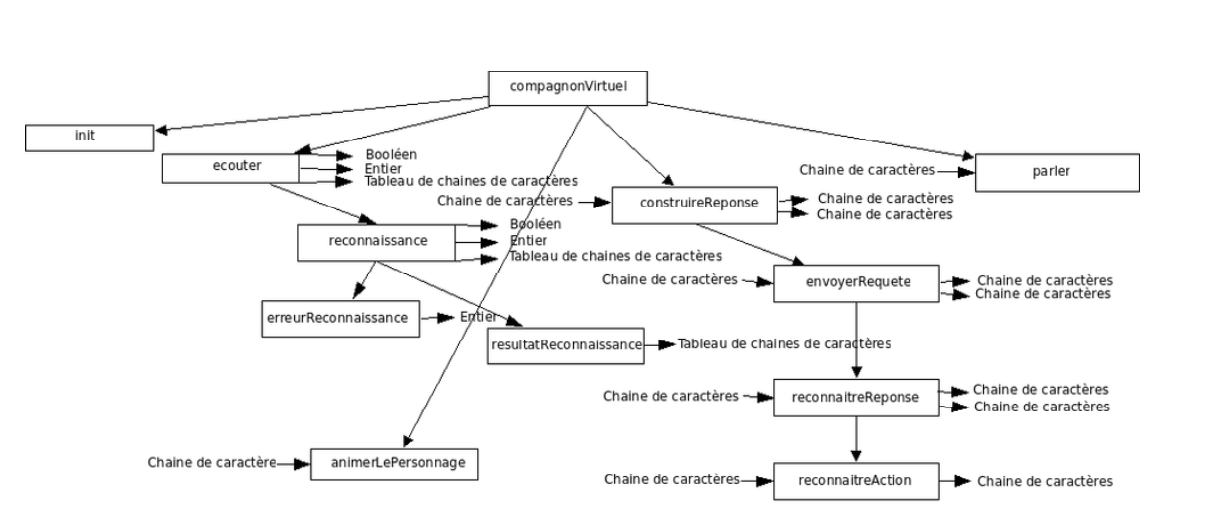
\includegraphics[width=1\linewidth]{analyseDescendante.png}
\caption{Analyse descendante de la version ancienne.\label{fig1}}
\end{figure}
\indent L'analyse descendante a été décrit dans le rapport  de 1ère version.
\newpage
